
\begin{frame}{Summary}
		\begin{figure}[ht]
			\begin{minipage}[b]{0.3\linewidth}
				\centering
				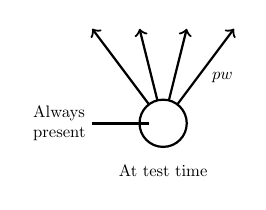
\begin{tikzpicture}[scale=.6, transform shape]
					\node[draw,thick,shape=circle,minimum width=1 cm] (A) at (2,0) {};
					\draw (0,0) node[text width=1.5cm] {Always present};
					\draw[line width=1pt] (0.5,0) -- (1.7,0);
					\draw[thick,->] (A) -- (0.5,2);
					\draw[thick,->] (A) -- (1.5,2);
					\draw[thick,->] (A) -- (2.5,2);
					\draw[thick,->] (A) -- (3.5,2) node[pos=.5,below right] {$pw$};
					\draw (2,-1) node[] {At test time};
				\end{tikzpicture}
				%\caption{Label for a}
				\label{fig:a}
			\end{minipage}
			\hspace{0.1cm}
			\begin{minipage}[b]{0.3\linewidth}
				\centering
				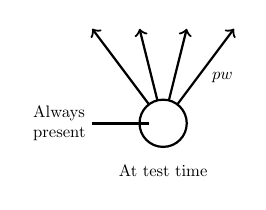
\begin{tikzpicture}[scale=.6, transform shape]
					\node[draw,thick,shape=circle,minimum width=1 cm] (A) at (2,0) {};
					\draw (0,0) node[text width=1.5cm] {Always present};
					\draw[line width=1pt] (0.5,0) -- (1.7,0);
					\draw[thick,->] (A) -- (0.5,2);
					\draw[thick,->] (A) -- (1.5,2);
					\draw[thick,->] (A) -- (2.5,2);
					\draw[thick,->] (A) -- (3.5,2) node[pos=.5,below right] {$pw$};
					\draw (2,-1) node[] {At test time};
				\end{tikzpicture}
				%\caption{Label for b}
				\label{fig:b}
			\end{minipage}
			\hspace{0.1cm}
			\begin{minipage}[b]{0.3\linewidth}
				\centering
				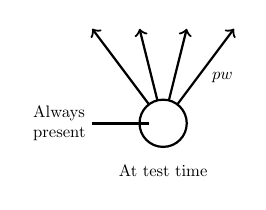
\begin{tikzpicture}[scale=.6, transform shape]
					\node[draw,thick,shape=circle,minimum width=1 cm] (A) at (2,0) {};
					\draw (0,0) node[text width=1.5cm] {Always present};
					\draw[line width=1pt] (0.5,0) -- (1.7,0);
					\draw[thick,->] (A) -- (0.5,2);
					\draw[thick,->] (A) -- (1.5,2);
					\draw[thick,->] (A) -- (2.5,2);
					\draw[thick,->] (A) -- (3.5,2) node[pos=.5,below right] {$pw$};
					\draw (2,-1) node[] {At test time};
				\end{tikzpicture}
				%\caption{Label for c}
				\label{fig:c}
			\end{minipage}
			\vspace{0.1cm}
			\begin{minipage}[b]{0.3\linewidth}
				\centering
				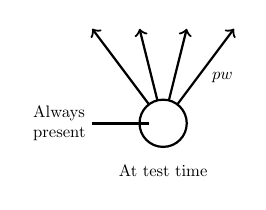
\begin{tikzpicture}[scale=.6, transform shape]
					\node[draw,thick,shape=circle,minimum width=1 cm] (A) at (2,0) {};
					\draw (0,0) node[text width=1.5cm] {Always present};
					\draw[line width=1pt] (0.5,0) -- (1.7,0);
					\draw[thick,->] (A) -- (0.5,2);
					\draw[thick,->] (A) -- (1.5,2);
					\draw[thick,->] (A) -- (2.5,2);
					\draw[thick,->] (A) -- (3.5,2) node[pos=.5,below right] {$pw$};
					\draw (2,-1) node[] {At test time};
				\end{tikzpicture}
				%\caption{Label for a}
				\label{fig:a}
			\end{minipage}
			\hspace{0.1cm}
			\begin{minipage}[b]{0.3\linewidth}
				\centering
				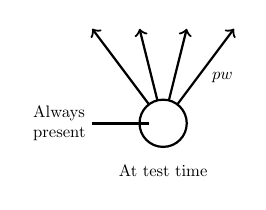
\begin{tikzpicture}[scale=.6, transform shape]
					\node[draw,thick,shape=circle,minimum width=1 cm] (A) at (2,0) {};
					\draw (0,0) node[text width=1.5cm] {Always present};
					\draw[line width=1pt] (0.5,0) -- (1.7,0);
					\draw[thick,->] (A) -- (0.5,2);
					\draw[thick,->] (A) -- (1.5,2);
					\draw[thick,->] (A) -- (2.5,2);
					\draw[thick,->] (A) -- (3.5,2) node[pos=.5,below right] {$pw$};
					\draw (2,-1) node[] {At test time};
				\end{tikzpicture}
				%\caption{Label for b}
				\label{fig:b}
			\end{minipage}
			\hspace{0.1cm}
			\begin{minipage}[b]{0.3\linewidth}
				\centering
				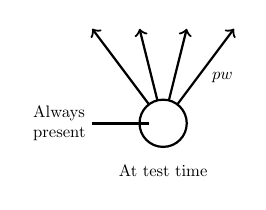
\begin{tikzpicture}[scale=.6, transform shape]
					\node[draw,thick,shape=circle,minimum width=1 cm] (A) at (2,0) {};
					\draw (0,0) node[text width=1.5cm] {Always present};
					\draw[line width=1pt] (0.5,0) -- (1.7,0);
					\draw[thick,->] (A) -- (0.5,2);
					\draw[thick,->] (A) -- (1.5,2);
					\draw[thick,->] (A) -- (2.5,2);
					\draw[thick,->] (A) -- (3.5,2) node[pos=.5,below right] {$pw$};
					\draw (2,-1) node[] {At test time};
				\end{tikzpicture}
				%\caption{Label for c}
				\label{fig:c}
			\end{minipage}
			\vspace{0.1cm}
			\begin{minipage}[b]{0.3\linewidth}
				\centering
				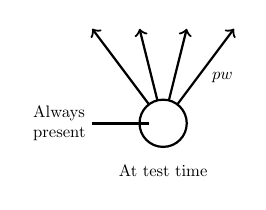
\begin{tikzpicture}[scale=.6, transform shape]
					\node[draw,thick,shape=circle,minimum width=1 cm] (A) at (2,0) {};
					\draw (0,0) node[text width=1.5cm] {Always present};
					\draw[line width=1pt] (0.5,0) -- (1.7,0);
					\draw[thick,->] (A) -- (0.5,2);
					\draw[thick,->] (A) -- (1.5,2);
					\draw[thick,->] (A) -- (2.5,2);
					\draw[thick,->] (A) -- (3.5,2) node[pos=.5,below right] {$pw$};
					\draw (2,-1) node[] {At test time};
				\end{tikzpicture}
				%\caption{Label for a}
				\label{fig:a}
			\end{minipage}
			\hspace{0.1cm}
			\begin{minipage}[b]{0.3\linewidth}
				\centering
				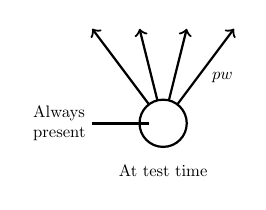
\begin{tikzpicture}[scale=.6, transform shape]
					\node[draw,thick,shape=circle,minimum width=1 cm] (A) at (2,0) {};
					\draw (0,0) node[text width=1.5cm] {Always present};
					\draw[line width=1pt] (0.5,0) -- (1.7,0);
					\draw[thick,->] (A) -- (0.5,2);
					\draw[thick,->] (A) -- (1.5,2);
					\draw[thick,->] (A) -- (2.5,2);
					\draw[thick,->] (A) -- (3.5,2) node[pos=.5,below right] {$pw$};
					\draw (2,-1) node[] {At test time};
				\end{tikzpicture}
				%\caption{Label for b}
				\label{fig:b}
			\end{minipage}
			\hspace{0.1cm}
			\begin{minipage}[b]{0.3\linewidth}
				\centering
				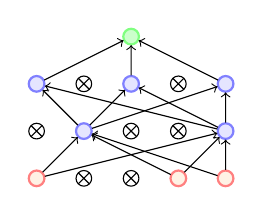
\begin{tikzpicture}[scale=.6, transform shape,cross/.style={path picture={ 
							\draw[black]
							(path picture bounding box.south east) -- (path picture bounding box.north west) (path picture bounding box.south west) -- (path picture bounding box.north east);
						}}]]
						\tikzstyle{input_neuron}=[circle,draw=red!50,fill=orange!10,thick,minimum size=.2mm]
						\tikzstyle{hidden_neuron}=[circle,draw=blue!50,fill=blue!10,thick,minimum size=1mm]
						\tikzstyle{output_neuron}=[circle,draw=green!50,fill=green!20,thick,minimum size=1mm]
																
						\tikzstyle{input}=[circle,draw=black!50,fill=black!20,thick,minimum size=.2mm]
						\tikzstyle{mynode} = [draw,shape=circle]
						\tikzstyle{mycross} = [draw,shape=circle,cross]
						\node[input_neuron,mynode] (a0) at (0, 0) {};
						\node[mycross] (a1) at (1, 0) {};
						\node[mycross] (a2) at (2, 0) {};
						\node[input_neuron,mynode] (a3) at (3, 0) {};
						\node[input_neuron,mynode] (a4) at (4, 0) {};
						\node[mycross] (b0) at (0, 1) {};
						\node[hidden_neuron,mynode] (b1) at (1, 1) {};
						\node[mycross] (b2) at (2, 1) {};
						\node[mycross] (b3) at (3, 1) {};
						\node[hidden_neuron,mynode] (b4) at (4, 1) {};
						\node[hidden_neuron,mynode] (c0) at (0, 2) {};
						\node[mycross] (c1) at (1, 2) {};
						\node[hidden_neuron,mynode] (c2) at (2, 2) {};
						\node[mycross] (c3) at (3, 2) {};
						\node[hidden_neuron,mynode] (c4) at (4, 2) {};
						\node[output_neuron,mynode] (d2) at (2, 3) {};
						\foreach \from in {a0,a3,a4}
						\foreach \to in {b1,b4}
						\draw [->] (\from) -- (\to);
						\foreach \from in {b1,b4}
						\foreach \to in {c0,c2,c4}
						\draw [->] (\from) -- (\to);
						\foreach \from in {c0,c2,c4}
						\draw [->] (\from) -- (d2);
					\end{tikzpicture}
					%\caption{Label for c}
					\label{fig:c}
				\end{minipage}
			\end{figure}
		\end{frame}